\begin{figure}[!t]
\begin{centering}
\tikzstyle{line} = [draw,  latex-]
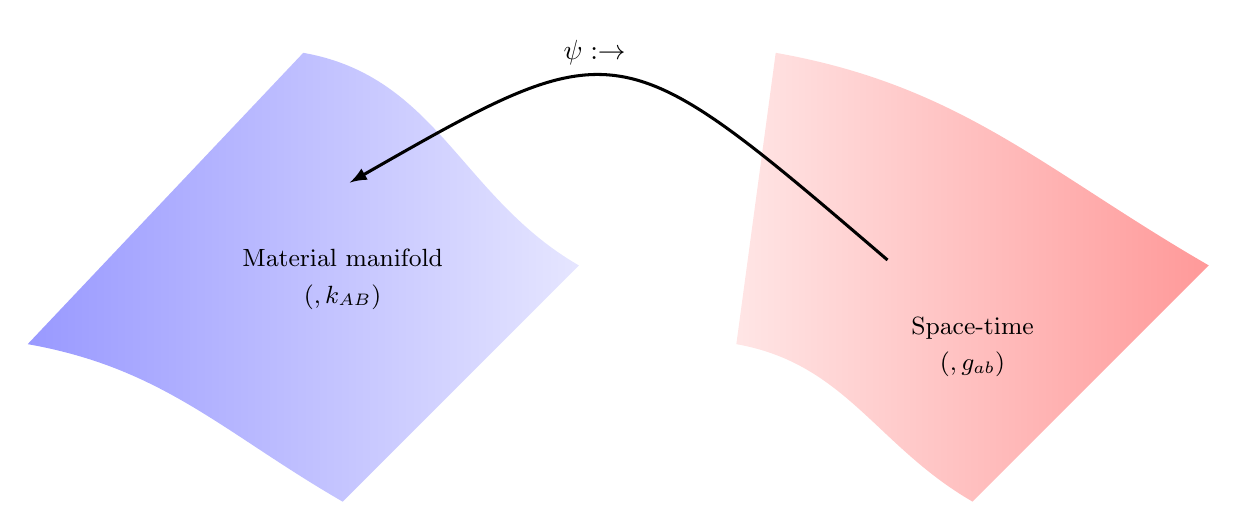
\begin{tikzpicture}
\shade[right color=blue!10,left color=blue!40] 
  (-1,0) to[out=-10,in=150] (3,-2) -- (6,1) to[out=150,in=-10] (2.5,3.7) -- cycle;
  \shade[left color=red!10,right color=red!40] 
  (8,0) to[out=-10,in=150] (11,-2) -- (14,1) to[out=150,in=-10] (8.5,3.7) -- cycle;
  % draw the map
\draw[line,black,line width=1.1pt,shorten >= 3pt,shorten <= 3pt] 
  (3,2) .. controls (6.5,4)   .. (10,1);
 
% we add some labels
\node[font=\color{black}] at (3,1.1) {{\small Material manifold}};
\node[font=\color{black}] at (3,0.6) {{\small $(\matmanif, k_{AB})$}};
\node[font=\color{black}] at (11,0.2) {{\small Space-time}};
\node[font=\color{black}] at (11,-0.25) {{\small$(\stmanif, g_{ab})$}};
\node[font=\color{black}] at (6.2,3.7) {$\psi:\stmanif \rightarrow \matmanif$}; 
\end{tikzpicture}
\caption{Schematic depiction of the  map $\psi$ that associates a point in the material space $\matmanif$ with a point in space-time $\stmanif$. We have also shown which metric is associated with which manifold (and the associated labelling of the indices).}\label{fig:shem_map}
\end{centering}
\end{figure}